% ============================================================
%  DISCOVERY CURRICULUM — Journey 4, Module 4
%  "Quantum Mechanics"
%  Compile with: pdflatex J4_M4.tex  (run twice)
% ============================================================
\documentclass[12pt,a4paper]{article}
\usepackage[a4paper,top=2.5cm,bottom=2.5cm,left=2.8cm,right=2.8cm,headheight=15pt]{geometry}
\usepackage{amsmath,amssymb,amsthm}
\usepackage{xcolor}
\usepackage{mdframed}
\usepackage{enumitem}
\usepackage{tikz}
\usetikzlibrary{arrows.meta,calc}
\usepackage{pgfplots}
\pgfplotsset{compat=1.18}
\usepackage{booktabs}
\usepackage{fancyhdr}
\usepackage{titlesec}
\usepackage{parskip}
\usepackage{hyperref}
\hypersetup{colorlinks=true,linkcolor=NavyBlue,urlcolor=NavyBlue}

\definecolor{NavyBlue}{HTML}{1A3A5C}
\definecolor{MidBlue}{HTML}{2E6DA4}
\definecolor{Gold}{HTML}{C8922A}
\definecolor{LightBlue}{HTML}{EBF2FA}
\definecolor{LightGold}{HTML}{FDF4E3}
\definecolor{DarkGrey}{HTML}{3A3A3A}
\definecolor{BoxGreen}{HTML}{E8F5E9}
\definecolor{SidebarGrey}{HTML}{F5F5F5}

\titleformat{\section}{\Large\bfseries\color{NavyBlue}}{}{0em}{}[{\color{MidBlue}\vspace{2pt}\rule{\linewidth}{1.5pt}}]
\titleformat{\subsection}{\large\bfseries\color{MidBlue}}{}{0em}{}

\pagestyle{fancy}\fancyhf{}
\fancyhead[L]{\small\color{DarkGrey}\textit{Discovery Curriculum}}
\fancyhead[R]{\small\color{DarkGrey}\textit{Journey 4 $\cdot$ Module 4}}
\fancyfoot[C]{\small\color{MidBlue}\thepage}
\renewcommand{\headrulewidth}{0.4pt}

\newmdenv[backgroundcolor=NavyBlue!7,linecolor=NavyBlue,linewidth=2pt,leftline=true,rightline=false,topline=false,bottomline=false,innerleftmargin=14pt,innerrightmargin=10pt,innertopmargin=10pt,innerbottommargin=10pt,skipabove=14pt,skipbelow=10pt]{puzzlebox}
\newmdenv[backgroundcolor=LightGold,linecolor=Gold,linewidth=2pt,leftline=true,rightline=false,topline=false,bottomline=false,innerleftmargin=14pt,innerrightmargin=10pt,innertopmargin=10pt,innerbottommargin=10pt,skipabove=14pt,skipbelow=10pt]{discoverybox}
\newmdenv[backgroundcolor=LightBlue,linecolor=MidBlue,linewidth=1.5pt,roundcorner=4pt,innerleftmargin=14pt,innerrightmargin=10pt,innertopmargin=10pt,innerbottommargin=10pt,skipabove=14pt,skipbelow=10pt]{namebox}
\newmdenv[backgroundcolor=BoxGreen,linecolor=DarkGrey!35,linewidth=1pt,roundcorner=4pt,innerleftmargin=14pt,innerrightmargin=10pt,innertopmargin=10pt,innerbottommargin=10pt,skipabove=14pt,skipbelow=10pt]{reflectionbox}
\newmdenv[backgroundcolor=SidebarGrey,linecolor=Gold,linewidth=1.2pt,leftline=true,rightline=false,topline=false,bottomline=false,innerleftmargin=12pt,innerrightmargin=10pt,innertopmargin=7pt,innerbottommargin=7pt,skipabove=10pt,skipbelow=10pt]{thought}

\newcounter{problem}
\newenvironment{problem}[1][]{\refstepcounter{problem}\par\vspace{6pt}\noindent\textbf{\color{MidBlue}Problem \theproblem}\ifx&#1&\else\ \textit{(#1)}\fi\textbf{.}\enskip}{\par\vspace{4pt}}
\newcounter{deepproblem}
\newenvironment{deepproblem}[1][]{\refstepcounter{deepproblem}\par\vspace{6pt}\noindent\textbf{\color{NavyBlue}$\bigstar$\ Deep Problem \thedeepproblem}\ifx&#1&\else\ \textit{(#1)}\fi\textbf{.}\enskip}{\par\vspace{4pt}}

\begin{document}

\thispagestyle{empty}
\begin{center}
{\small\color{MidBlue}\textbf{DISCOVERY CURRICULUM}\quad$\cdot$\quad\textbf{JOURNEY 4: FIELDS AND SPACE}}
\vspace{0.6cm}

{\color{NavyBlue}\rule{\linewidth}{2pt}}\vspace{0.5cm}

{\Huge\bfseries\color{NavyBlue}Module 4}\\[0.3cm]
{\LARGE\bfseries\color{MidBlue}Quantum Mechanics}\\[0.4cm]
{\color{Gold}\rule{0.4\linewidth}{1.2pt}}\\[0.4cm]
{\large\itshape\color{DarkGrey}
The Schr\"{o}dinger equation is the heat equation\\[0.15cm]
with an imaginary diffusion constant. That one change\\[0.15cm]
makes everything different.}

\vspace{1cm}
\begin{tabular}{rl}
\color{DarkGrey}\textbf{Journey}         & Journey 4 --- Fields and Space \\[4pt]
\color{DarkGrey}\textbf{Module}          & 4 of 6 \\[4pt]
\color{DarkGrey}\textbf{Prerequisites}   & J4 Modules 1--3; J3 Modules 3, 5 \\[4pt]
\color{DarkGrey}\textbf{You will discover} & Schr\"{o}dinger equation, wave functions, energy levels, hydrogen atom, spin \\[4pt]
\color{DarkGrey}\textbf{Format}          & 8 problems $+$ 3 deep problems $\approx$ 15 pages \\
\end{tabular}
\vspace{1cm}

{\color{NavyBlue}\rule{\linewidth}{2pt}}
\end{center}

\vspace{0.5cm}
\noindent\textbf{The quantum revolution.}
Classical mechanics failed in three domains: atomic spectra (atoms emit only specific frequencies of light), the photoelectric effect (light ejects electrons only above a threshold frequency), and the stability of atoms (classically, an electron orbiting a nucleus should spiral in and radiate away all its energy in microseconds). Quantum mechanics resolved all three by a single radical idea: energy is quantised, and particles are described by complex-valued wave functions whose modulus squared gives probability.

\medskip
The mathematics is everything from Journeys 2--4: the Schr\"{o}dinger equation is a PDE; its solutions are eigenfunctions of the Hamiltonian operator; the eigenvalues are energy levels; the spectral theorem (Journey~3) guarantees they are real; and physical predictions are computed from inner products.

\newpage

\section{Part 1 \texorpdfstring{---}{--} The Puzzle}

\begin{puzzlebox}
\textbf{The Opening Puzzle: The particle in a box.}

An electron is trapped between $x=0$ and $x=L$ (infinite potential walls). The time-independent Schr\"{o}dinger equation inside is $-\frac{\hbar^2}{2m}\psi''(x) = E\psi(x)$ with $\psi(0)=\psi(L)=0$.

\medskip
\textbf{Question 1.} This is an eigenvalue problem. What type of ODE is it? You have solved this before.

\textbf{Question 2.} Find all solutions satisfying the boundary conditions. What values of $E$ are allowed? Write a formula for $E_n$.

\textbf{Question 3.} Can $E=0$? Why not? What physical principle does this represent?

\textbf{Question 4.} Normalise the solution: find $A$ such that $\int_0^L|\psi_n(x)|^2\,dx=1$.

\textbf{Question 5.} Sketch $|\psi_n|^2$ for $n=1,2,3$. How does the number of nodes relate to $n$? To the energy?
\end{puzzlebox}

\section{Part 2 \texorpdfstring{---}{--} Exploration}

\subsection{Step 1: The Schr\"{o}dinger equation}

\begin{problem}
\label{prob:schrodinger}
\begin{enumerate}[label=(\alph*),topsep=2pt]
  \item The \textbf{time-dependent Schr\"{o}dinger equation} is $i\hbar\partial_t\psi = H\psi$ where $H = -\frac{\hbar^2}{2m}\nabla^2 + V(\mathbf{x})$ is the Hamiltonian operator. Separate $\psi(\mathbf{x},t) = \phi(\mathbf{x})e^{-iEt/\hbar}$ to derive the time-independent equation $H\phi = E\phi$.
  \item Show that if $\psi$ satisfies the Schr\"{o}dinger equation, then $\partial_t|\psi|^2 + \nabla\cdot\mathbf{J} = 0$ where $\mathbf{J} = \frac{\hbar}{2mi}(\psi^*\nabla\psi - \psi\nabla\psi^*)$ is the \textbf{probability current}. This is conservation of probability.
  \item The total probability $\int|\psi|^2\,dV=1$ is preserved in time (unitary evolution). Show this follows from the fact that $H$ is self-adjoint and $e^{-iHt/\hbar}$ is unitary.
  \item The \textbf{expected value} of an observable $A$ in state $\psi$ is $\langle A\rangle = \int\psi^* A\psi\,dV = \langle\psi,A\psi\rangle$. Compute $\langle x\rangle$ and $\langle p\rangle$ (where $p=-i\hbar\partial_x$) for $\psi_n(x) = \sqrt{2/L}\sin(n\pi x/L)$ (particle in a box).
  \item Show: if $\psi$ is an eigenstate of $H$ with eigenvalue $E$, then $\langle H\rangle = E$ and $\Delta H = 0$ (zero uncertainty in energy). An energy eigenstate has perfectly definite energy.
\end{enumerate}
\end{problem}

\begin{thought}
\textbf{What is the wave function?}
The wave function $\psi(x,t)$ is a complex-valued function. Its modulus squared $|\psi(x,t)|^2$ gives the probability density of finding the particle at position $x$ at time $t$. This is Born's rule (1926). $\psi$ itself is not directly observable --- only $|\psi|^2$ is. Yet $\psi$ is the central object of the theory, and quantum mechanics cannot be formulated without it. The wave function represents the state of a system: all physically meaningful information about the system is encoded in $\psi$. What $\psi$ \emph{is} --- whether it is a physical wave in space, a mathematical bookkeeping device, or something else entirely --- is the measurement problem of quantum mechanics, which remains philosophically unresolved.
\end{thought}

\subsection{Step 2: The quantum harmonic oscillator}

\begin{problem}
\label{prob:qho}
The \textbf{quantum harmonic oscillator} has $V(x)=\frac{1}{2}m\omega^2 x^2$ and Hamiltonian $H = -\frac{\hbar^2}{2m}\frac{d^2}{dx^2}+\frac{1}{2}m\omega^2 x^2$.

\begin{enumerate}[label=(\alph*),topsep=2pt]
  \item Change variables: let $\xi = x\sqrt{m\omega/\hbar}$ and $\varepsilon = 2E/(\hbar\omega)$. Show the equation becomes $-\psi''+\xi^2\psi = \varepsilon\psi$.
  \item For large $|\xi|$, the equation is approximately $\psi''\approx\xi^2\psi$, with decaying solution $e^{-\xi^2/2}$. Try $\psi(\xi) = H(\xi)e^{-\xi^2/2}$. Show $H$ satisfies the \textbf{Hermite equation}: $H''-2\xi H'+({\varepsilon-1})H=0$.
  \item For $\psi$ to be normalisable, $H$ must be a polynomial (the series solution must terminate). This forces $\varepsilon = 2n+1$ for $n=0,1,2,\ldots$, giving energy levels $E_n = \hbar\omega(n+\frac{1}{2})$.
  \item The \textbf{zero-point energy} $E_0=\frac{1}{2}\hbar\omega$ is non-zero even in the ground state. Interpret using the uncertainty principle: localising the particle to a potential well forces non-zero kinetic energy.
  \item The first three Hermite polynomials are $H_0=1$, $H_1=2\xi$, $H_2=4\xi^2-2$. Write out $\psi_0,\psi_1,\psi_2$ (unnormalised) and sketch them. Count nodes.
\end{enumerate}
\end{problem}

\begin{problem}
\label{prob:ladder}
\textbf{The ladder operator method.} Define $\hat{a} = \frac{1}{\sqrt{2m\hbar\omega}}\left(m\omega x + i\hat{p}\right)$ and $\hat{a}^\dagger = \frac{1}{\sqrt{2m\hbar\omega}}\left(m\omega x - i\hat{p}\right)$.
\begin{enumerate}[label=(\alph*),topsep=2pt]
  \item Show $[\hat{a},\hat{a}^\dagger] = 1$ (commutator equals identity).
  \item Show $H = \hbar\omega\left(\hat{a}^\dagger\hat{a}+\frac{1}{2}\right)$.
  \item Show: if $H\psi_n=E_n\psi_n$, then $\hat{a}^\dagger\psi_n$ is an eigenstate with energy $E_n+\hbar\omega$ (raising operator) and $\hat{a}\psi_n$ is an eigenstate with energy $E_n-\hbar\omega$ (lowering operator).
  \item The ground state satisfies $\hat{a}\psi_0=0$. Solve this first-order ODE to find $\psi_0(\xi) = Ce^{-\xi^2/2}$.
  \item The ladder operators are the quantum analogue of what classical concept? Why is this algebraic method (no solving differential equations!) so powerful?
\end{enumerate}
\end{problem}

\subsection{Step 3: The hydrogen atom}

\begin{problem}
\label{prob:hydrogen}
The hydrogen atom: a single electron ($m_e$, charge $-e$) orbiting a proton (charge $+e$). The Hamiltonian is $H = -\frac{\hbar^2}{2m_e}\nabla^2 - \frac{e^2}{4\pi\varepsilon_0 r}$.

\begin{enumerate}[label=(\alph*),topsep=2pt]
  \item Separate in spherical coordinates: $\psi(r,\theta,\phi) = R(r)Y(\theta,\phi)$. The angular part satisfies $-\nabla_{\text{angular}}^2 Y = \ell(\ell+1)Y$ (the spherical Laplacian eigenvalue problem). The solutions are the \textbf{spherical harmonics} $Y_\ell^m(\theta,\phi)$.
  \item The radial equation (after substitution $R = u(r)/r$) becomes:
  $-\frac{\hbar^2}{2m_e}u'' + \left[-\frac{e^2}{4\pi\varepsilon_0 r} + \frac{\hbar^2\ell(\ell+1)}{2m_e r^2}\right]u = Eu$.
  For bound states ($E<0$), show the energy levels are $E_n = -\frac{m_e e^4}{2(4\pi\varepsilon_0)^2\hbar^2 n^2} = -\frac{13.6\,\text{eV}}{n^2}$ for $n=1,2,3,\ldots$
  \item For each $n$: $\ell$ ranges from $0$ to $n-1$; $m$ ranges from $-\ell$ to $\ell$. Count the total number of states with energy $E_n$ (the degeneracy). For $n=3$, list all $(n,\ell,m)$ combinations.
  \item The ground state wave function is $\psi_{100} = \frac{1}{\sqrt{\pi a_0^3}}e^{-r/a_0}$ where $a_0 = \frac{4\pi\varepsilon_0\hbar^2}{m_e e^2} \approx 0.53$ \AA\/ is the Bohr radius. Verify normalisation.
  \item \textbf{Spectral lines.} A photon emitted in the transition $n\to n'$ has frequency $\nu = (E_n-E_{n'})/h$. For the Balmer series ($n'=2$, $n=3,4,5,6$): compute the four wavelengths. Three are in the visible range. Verify: $656\,\text{nm}$ (red), $486\,\text{nm}$ (blue-green), $434\,\text{nm}$ (violet), $410\,\text{nm}$ (deep violet).
\end{enumerate}
\end{problem}

\begin{center}
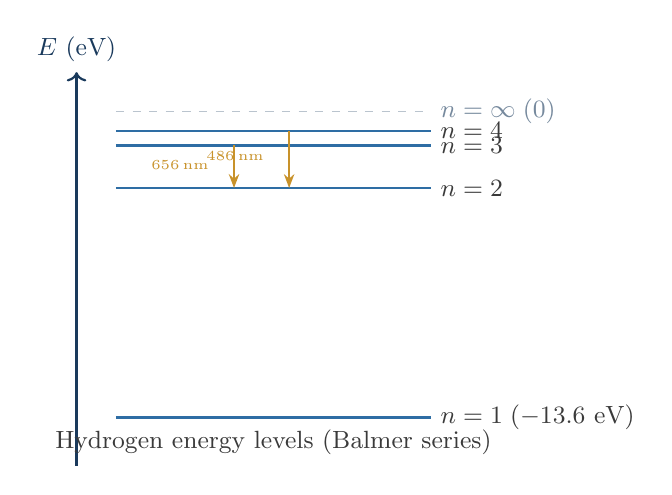
\begin{tikzpicture}
% Energy level diagram for hydrogen
\draw[NavyBlue,thick,->] (-0.5,-4.5) -- (-0.5,0.5) node[above,font=\small]{$E$ (eV)};
% Energy levels
\foreach \n/\E/\lbl in {1/-13.6/$n=1$\;$(-13.6\text{ eV})$, 2/-3.4/$n=2$, 3/-1.51/$n=3$, 4/-0.85/$n=4$}{
  \draw[MidBlue,thick] (0,{\E/3.5}) -- (4,{\E/3.5});
  \node[right,font=\small,color=DarkGrey] at (4,{\E/3.5}) {\lbl};
}
\draw[NavyBlue!30,dashed] (0,0) -- (4,0) node[right,font=\small,color=NavyBlue!60]{$n=\infty$\;$(0)$};
% Balmer transitions
\draw[-{Stealth[length=5pt]},Gold,thick] (1.5,{-1.51/3.5}) -- (1.5,{-3.4/3.5});
\node[Gold,font=\tiny,left] at (1.3,{-2.4/3.5}) {$656\,\text{nm}$};
\draw[-{Stealth[length=5pt]},Gold,thick] (2.2,{-0.85/3.5}) -- (2.2,{-3.4/3.5});
\node[Gold,font=\tiny,left] at (2.0,{-2.0/3.5}) {$486\,\text{nm}$};
\node[DarkGrey,font=\small] at (2,-4.2) {Hydrogen energy levels (Balmer series)};
\end{tikzpicture}
\end{center}

\subsection{Step 4: Spin and the Dirac equation}

\begin{problem}
\label{prob:spin}
\textbf{Spin.} Electrons have an intrinsic angular momentum called spin, described by a 2-component spinor $|\psi\rangle = \alpha|\uparrow\rangle + \beta|\downarrow\rangle$ with $|\alpha|^2+|\beta|^2=1$.
\begin{enumerate}[label=(\alph*),topsep=2pt]
  \item The spin operators are $S_i = \frac{\hbar}{2}\sigma_i$ where $\sigma_x,\sigma_y,\sigma_z$ are the \textbf{Pauli matrices}:
  $\sigma_x=\begin{pmatrix}0&1\\1&0\end{pmatrix}$, $\sigma_y=\begin{pmatrix}0&-i\\i&0\end{pmatrix}$, $\sigma_z=\begin{pmatrix}1&0\\0&-1\end{pmatrix}$.
  Compute $[\sigma_x,\sigma_y]$, $[\sigma_y,\sigma_z]$, $[\sigma_z,\sigma_x]$.
  \item The commutation relations are $[S_i,S_j]=i\hbar\epsilon_{ijk}S_k$. These are the structure constants of the Lie algebra $\mathfrak{su}(2)$. Verify for one pair.
  \item If a spin is in state $|\uparrow\rangle$ along $z$, what is the probability of measuring spin-up along $x$? (Apply $\sigma_x$ to $|\uparrow\rangle = (1,0)^T$ and decompose in the eigenbasis of $\sigma_x$.)
  \item \textbf{Stern-Gerlach experiment}: a beam of silver atoms passing through an inhomogeneous magnetic field splits into two discrete beams. Classical physics predicts a continuous smear. Explain the quantum explanation.
  \item \textbf{Entanglement}: two electrons in the singlet state $\frac{1}{\sqrt{2}}(|\uparrow\downarrow\rangle - |\downarrow\uparrow\rangle)$. If electron 1 is measured spin-up along $z$, what is the state of electron 2? Why does this not allow faster-than-light communication?
\end{enumerate}
\end{problem}

\begin{problem}
\label{prob:uncertainty}
\textbf{The uncertainty principle.}
\begin{enumerate}[label=(\alph*),topsep=2pt]
  \item For position $\hat{x}$ and momentum $\hat{p}=-i\hbar\partial_x$, compute $[\hat{x},\hat{p}]$ as an operator. Show $[\hat{x},\hat{p}]=i\hbar I$.
  \item The \textbf{Robertson uncertainty relation}: for any two observables $A,B$, $\Delta A\cdot\Delta B \geq \frac{1}{2}|\langle[A,B]\rangle|$. Derive the Heisenberg uncertainty principle $\Delta x\cdot\Delta p \geq \hbar/2$.
  \item For a Gaussian wave packet $\psi(x) = (2\pi\sigma^2)^{-1/4}e^{-x^2/4\sigma^2}$: compute $\Delta x$ and $\Delta p$. Show $\Delta x\cdot\Delta p = \hbar/2$ (the Gaussian saturates the uncertainty bound).
  \item The \textbf{energy-time uncertainty}: $\Delta E\cdot\Delta t \geq \hbar/2$. This is more subtle (time is not an operator in QM). Interpret: a state with finite lifetime $\tau$ has energy uncertainty $\Delta E \sim \hbar/\tau$. This explains the finite linewidth of spectral lines.
  \item Connect to the Fourier transform: $\Delta x$ is the width of $\psi(x)$ and $\Delta p/\hbar$ is the width of $\hat\psi(k)$ (its Fourier transform). The uncertainty principle is simply the Fourier bandwidth theorem: a function and its Fourier transform cannot both be sharply localised.
\end{enumerate}
\end{problem}

\section{Part 3 \texorpdfstring{---}{--} Discovery}

\begin{discoverybox}
\textbf{What have we built?}

\textbf{First.} The Schr\"{o}dinger equation $i\hbar\partial_t\psi = H\psi$ is a linear PDE. Its stationary solutions are eigenfunctions of $H$; the eigenvalues are the quantised energy levels. The spectral theorem guarantees real eigenvalues; unitarity guarantees probability conservation.

\textbf{Second.} Every physical system's quantum mechanics reduces to finding the eigenfunctions and eigenvalues of its Hamiltonian. The particle in a box, the harmonic oscillator, and the hydrogen atom are the three fundamental solved systems, and they involve (respectively) sine functions, Hermite polynomials, and spherical harmonics times radial functions.

\textbf{Third.} The uncertainty principle is not a measurement disturbance --- it is a fundamental property of wave functions related to the non-commutativity of position and momentum operators. It is the Fourier uncertainty principle in disguise.

\textbf{Fourth.} Spin is an intrinsic quantum degree of freedom described by the algebra of $2\times 2$ matrices (Pauli matrices) and the Lie algebra $\mathfrak{su}(2)$. It has no classical analogue.

\medskip
\textbf{The thread forward.} The hydrogen atom's energy levels depend only on $n$, but the wave functions carry additional quantum numbers $\ell,m$. This degeneracy is a consequence of the additional symmetry of the Coulomb potential (it has $SO(4)$ symmetry, not just $SO(3)$). Symmetry and degeneracy are intimately connected --- a theme that Journey~7 will develop systematically through group theory.
\end{discoverybox}

\section{Part 4 \texorpdfstring{---}{--} Naming the Ideas}

\begin{namebox}
\textbf{Quantum mechanics --- postulates.}

\textbf{1. State}: the quantum state is a normalised vector $|\psi\rangle$ in a Hilbert space $\mathcal{H}$.

\textbf{2. Observables}: physical observables are self-adjoint operators on $\mathcal{H}$.

\textbf{3. Born rule}: measuring observable $A$ in state $|\psi\rangle$ gives eigenvalue $\lambda_i$ with probability $|\langle\phi_i|\psi\rangle|^2$ where $|\phi_i\rangle$ is the corresponding eigenstate.

\textbf{4. Collapse}: after measuring eigenvalue $\lambda_i$, the state collapses to $|\phi_i\rangle$.

\textbf{5. Evolution}: between measurements, $i\hbar\partial_t|\psi\rangle = H|\psi\rangle$; equivalently $|\psi(t)\rangle = e^{-iHt/\hbar}|\psi(0)\rangle$.
\end{namebox}

\section{Part 5 \texorpdfstring{---}{--} Deep Problems}

\begin{deepproblem}[Path integrals]
Feynman's formulation: the quantum amplitude for a particle to go from $(x_a,t_a)$ to $(x_b,t_b)$ is
\[
  K(x_b,t_b;x_a,t_a) = \int\mathcal{D}[x(t)]\,e^{iS[x]/\hbar},
\]
where the integral is over all paths $x(t)$ from $x_a$ to $x_b$, and $S[x]=\int_{t_a}^{t_b}L(x,\dot x)\,dt$ is the classical action.
\begin{enumerate}[label=(\alph*)]
  \item In the limit $\hbar\to 0$, the exponential oscillates rapidly for all paths except the one with stationary action $\delta S=0$. Show this recovers the classical Euler-Lagrange equation. The path integral contains classical mechanics as a limit.
  \item For a free particle ($V=0$), the path integral can be computed exactly. Discretise the path into $N$ steps and compute the Gaussian integrals; take $N\to\infty$. The result is $K = \sqrt{\frac{m}{2\pi i\hbar(t_b-t_a)}}\exp\left(\frac{im(x_b-x_a)^2}{2\hbar(t_b-t_a)}\right)$.
  \item Compare with the heat kernel from Module~3: the free quantum propagator is the heat kernel with $t\to it/\hbar$ (imaginary time). This is the \textbf{Wick rotation}. What does it mean to continue to imaginary time?
  \item The path integral approach extends to quantum field theory (QFT): fields replace particles, and the path integral is over all field configurations. In QFT, the Wick-rotated path integral gives a statistical mechanics partition function. Write one sentence on why the connection between quantum mechanics and statistical mechanics is not a coincidence.
\end{enumerate}
\end{deepproblem}

\begin{deepproblem}[The Dirac equation and relativistic quantum mechanics]
The Schr\"{o}dinger equation is non-relativistic. The \textbf{Dirac equation} combines quantum mechanics with special relativity:
\[
  (i\hbar\gamma^\mu\partial_\mu - mc)\psi = 0,
\]
where $\psi$ is a 4-component spinor and $\gamma^\mu$ are $4\times 4$ matrices satisfying $\{\gamma^\mu,\gamma^\nu\}=2g^{\mu\nu}$ (Clifford algebra).
\begin{enumerate}[label=(\alph*)]
  \item Show the Dirac equation implies the Klein-Gordon equation $(\Box + m^2c^2/\hbar^2)\psi=0$ by applying $(i\hbar\gamma^\mu\partial_\mu+mc)$ from the left.
  \item The Dirac equation has both positive-energy solutions (electrons) and negative-energy solutions. Dirac interpreted negative-energy states as a filled sea of electrons; the absence of a negative-energy electron appears as a positron (antiparticle). This prediction of antimatter was confirmed experimentally in 1932. What mathematical feature of the equation forced Dirac to predict antimatter?
  \item The Pauli matrices appear as a sub-structure of the gamma matrices. Show this and explain why spin emerges naturally from the Dirac equation (it is not postulated separately, unlike in non-relativistic QM).
  \item The hydrogen atom energy levels from the Dirac equation include relativistic corrections: $E_{n\ell j} = -\frac{13.6\,\text{eV}}{n^2}\left[1+\frac{\alpha^2}{n^2}\left(\frac{n}{j+1/2}-\frac{3}{4}\right)+\cdots\right]$ where $\alpha\approx1/137$ is the fine structure constant. The extra quantum number $j$ is the total angular momentum. Explain qualitatively where this fine structure comes from.
\end{enumerate}
\end{deepproblem}

\begin{deepproblem}[Quantum information and entanglement]
\begin{enumerate}[label=(\alph*)]
  \item A \textbf{qubit} is a quantum state $\alpha|0\rangle+\beta|1\rangle$ with $|\alpha|^2+|\beta|^2=1$. The state space is the Bloch sphere $S^2 = \mathbb{CP}^1$. Describe the Bloch sphere and identify which points correspond to the classical states $|0\rangle$ and $|1\rangle$, and to superpositions.
  \item \textbf{Bell's theorem}: the singlet state $\frac{1}{\sqrt{2}}(|01\rangle-|10\rangle)$ produces correlations between measurements on the two qubits that cannot be reproduced by any local hidden variable theory. The \textbf{CHSH inequality} $|E(a,b)-E(a,b')+E(a',b)+E(a',b')|\leq 2$ is satisfied by all classical theories but violated by quantum mechanics (maximum $2\sqrt{2}$). This is experimental proof that nature is non-local. Compute the quantum value for optimal measurement angles.
  \item \textbf{Quantum teleportation}: using a shared entangled pair, Alice can transmit an unknown quantum state to Bob using only classical communication. The protocol uses Bell state measurements and conditional unitary operations. Describe the protocol and identify what information is sent classically and what is not.
  \item The \textbf{no-cloning theorem}: there is no unitary operation $U$ such that $U|\psi\rangle|0\rangle = |\psi\rangle|\psi\rangle$ for all $|\psi\rangle$. Prove this using the linearity of quantum mechanics. What is the classical analogue and why does it hold classically?
\end{enumerate}
\end{deepproblem}

\section{Part 6 \texorpdfstring{---}{--} Reflection}

\begin{reflectionbox}
\textbf{Your reflection task.}

\begin{enumerate}
  \item \textbf{On the measurement problem.} The wave function evolves deterministically under the Schr\"{o}dinger equation, but measurement produces a definite outcome and ``collapses'' the wave function. These two processes seem incompatible. Write a paragraph: is this a problem with the theory, or a problem with our interpretation of the theory?

  \item \textbf{On quantisation.} The energy levels of the hydrogen atom are $E_n=-13.6/n^2$ eV, discrete and countable. Yet classically, an electron can orbit at any energy. Write: why does confinement force discreteness? Is this a special property of quantum mechanics, or does something similar happen in classical wave physics?

  \item \textbf{On the unreasonable applicability of linear algebra.} Quantum mechanics is linear algebra on an infinite-dimensional Hilbert space. Observables are self-adjoint operators; states are unit vectors; measurements are projections; time evolution is unitary. The entire structure you built in Journey~3 applies directly. Write a paragraph: does this feel like a coincidence, or does it suggest something about why the universe is structured the way it is?

  \item \textbf{Looking ahead.} Module~5 studies classical mechanics through Hamilton's principle of least action. You saw in Module~4 of Journey~2 (Snell's law as a minimisation principle) and here (the path integral recovers classical mechanics in the limit $\hbar\to 0$) that variational principles unify large areas of physics. What do you expect the action functional to be?
\end{enumerate}
\end{reflectionbox}

\medskip
\noindent\textbf{Looking ahead.}
Module~5 studies Lagrangian and Hamiltonian mechanics: the variational formulation of classical physics that naturally generalises to quantum mechanics, field theory, and relativity. The principle of least action is the deepest formulation of classical mechanics and the starting point for every modern physical theory.

\vspace{1.4cm}
\begin{center}
{\color{MidBlue}\rule{0.5\linewidth}{0.8pt}}\\[6pt]
{\small\color{DarkGrey}\textit{End of Journey 4, Module 4 --- Quantum Mechanics}}\\[4pt]
{\small\color{DarkGrey}Continue to: \textbf{Module 5 --- Classical Mechanics and the Principle of Least Action}}\\[6pt]
{\color{MidBlue}\rule{0.5\linewidth}{0.8pt}}
\end{center}

\end{document}